%! Author = danielmendes
%! Date = 26.01.25

\chapter{Views}\label{ch:views}
Im folgenden Kapitel betrachten wir die Performance Vorteile von Sichten (engl.\ Views) in SQL\@.
Zunächst befassen wir uns mit virtuellen Sichten, ihren Vor- und Nachteilen sowie dem Verhalten bei Inserts.
Danach widmen wir uns materialisierten Sichten, die physisch in der Datenbank gespeichert werden, und deren Implementierung.
Dabei erklären und nutzen wir Trigger, da MySQL keine native Unterstützung für materialisierte Sichten bietet.
In den letzten beiden Kapiteln betrachten wir die Durchführung der Benchmarks näher und interpretieren die entstandenen Ergebnisse.

\section{Virtuelle Views}\label{sec:virtuelle-views}

Grundlegend existieren Relationen, bzw.\ Tabellen, die durch das \texttt{CREATE TABLE} – Statement definiert werden, physisch in der Datenbank.
Damit sind sie persistent, was bedeutet, dass sie dauerhaft existieren und sich nicht ändern, es sei denn, sie werden explizit durch eine SQL-Änderungsanweisung dazu aufgefordert.
Dies entspricht der Dauerhaftigkeit des ACID-Prinzips~\cite{acid_eigenschaften}, die sicherstellt, dass bestätigte Transaktionen dauerhaft gespeichert bleiben und auch bei Systemausfällen nicht verloren gehen.
Es gibt jedoch eine weitere Klasse von SQL-Relationen, die nicht wie Tabellen physisch gespeichert werden (\cite[341--349, 353--366]{garcia2008database}, ~\cite[pp. 276--281]{schwartz2012high}).
Sie werden als virtuelle Sichten bezeichnet.
Virtuelle Sichten werden durch einen Ausdruck definiert, der einer Abfrage ähnelt und können auch so abgefragt werden, als ob sie tatsächlich physisch existierten.
In einigen Fällen kann man sogar die Datensätze über die Sicht geändert werden.
\vspace{-5pt}
\begin{lstlisting}[language=SQL,caption=Allgemeine View-Deklaration,label={lst:create_view}]
CREATE VIEW <name> AS <definition>;
\end{lstlisting}
\vspace{-5pt}

In dem Codeblock~\ref{lst:create_view} sehen wir die Struktur der Definition einer View.
Als Nächstes müssen wir die \texttt{view-definition} mit einer SQL-Abfrage ersetzen, die den Inhalt der virtuellen Sicht abbilden soll.
Um dieses Vorgehen mit einem Beispiel näher zu veranschaulichen, nutzen wir die Tabellen Kunden (\ref{lst:tools-create-table-kunde}) und Bestellung (\ref{lst:tools-create-table-bestellung}).
Nun wollen wir, dass die beiden Tabellen über die \texttt{KUNDEN\_ID} in der Sicht zusammengefügt werden, da die \texttt{KUNDEN\_ID} zum einen der Primärschlüssel der Kundentabelle ist und zum anderen der Fremdschlüssel in Bestellung.
Um in die SQL-Abfrage noch etwas mehr Komplexität zu bekommen, wollen wir neben der Join-Operation zusätzlich den Umsatz pro Jahr und pro Stadt aggregieren.
Diese Aggregation könnte beispielsweise von einem Marketingteam genutzt werden, um schwache Regionen zu identifizieren und gezielt in diesen nachzusteuern.
Die View mit dem Namen \texttt{KUNDEN\_OVERVIEW} hat folgende Struktur:

\vspace{-5pt}
\lstinputlisting[
    language=sql,
    caption=View Deklarierung,
    label={lst:create_kunden_bestellung_view},
    style=custom_daniel,
]{Scripts/Views/01_create_view.sql}

Wenn wir die Daten dieser virtuellen Sicht abfragen wollen, dann adressieren wir den Namen in der FROM-Klausel und verlassen uns darauf, dass das Datenbankmanagementsystem die benötigten Tupel erzielt (siehe~\ref{lst:select-view}).
Dabei operiert das DBMS direkt auf den Relationen, die die virtuelle Sicht definieren.
In unserem Fall sind das die Kunden- und Bestelltabelle.

\vspace{-5pt}
\begin{lstlisting}[language=SQL,caption=SQL-Befehl mit Sicht,label={lst:select-view}]
SELECT * FROM KUNDEN_OVERVIEW
ORDER BY Jahr ASC, Gesamtumsatz DESC;
\end{lstlisting}
\vspace{-5pt}

Eine weitere Möglichkeit, die Funktionsweise einer Sicht besser zu verstehen, besteht darin, sie in einer FROM-Klausel durch eine Unterabfrage zu ersetzen, die identisch mit der Sichtdefinition ist.
Die Unterabfrage müssen wir noch mit einer Tupelvariablen ergänzen, damit wir auch Bezug auf die Tupel nehmen können.
Die SQL-Abfrage aus~\ref{lst:select-without-view} liefert das gleiche Ergebnis wie die aus~\ref{lst:select-view}, wenn wir unsere View wie im Beispiel~\ref{lst:create_kunden_bestellung_view} definieren.
Zu dem Einfluss auf die Performance kommen wir in den späteren Unterkapiteln \nameref{sec:durchfuhrung-der-benchmarks} und \nameref{sec:analyse-der-ergebnisse}.

\lstinputlisting[
    language=sql,
    caption=Select-Befehl ohne Sicht,
    label={lst:select-without-view},
    style=custom_daniel,
]{Scripts/Views/02_select_without_view.sql}

Man kann den Attributen einer Sicht eigene Namen vergeben, indem man sie in Klammern hinter dem Namen der Sicht aus der \texttt{CREATE VIEW}-Anweisung auflistet.
Die Definition einer Sicht kann mit \texttt{DROP VIEW <view-name>} gelöscht werden, wodurch keine Abfragen mehr auf dieser Sicht ausgeführt werden können.
Das Löschen der Sicht hat jedoch keine Auswirkungen auf die Tupel der zugrundeliegenden Tabellen.
Im Gegensatz dazu würde \texttt{DROP TABLE <table-name>} die Tabelle löschen und damit auch die darauf basierenden Sichten unbrauchbar machen, da ihre Definitionen auf der gelöschten Tabelle beruhen.

Abgesehen vom Löschen der Tabellen kann man auch Einfügungen an der View durchführen.
Dies ist aber nicht uneingeschränkt möglich und nur unter bestimmten Bedingungen erlaubt.
Zum einen muss die Sicht durch eine einfache Abfrage aus nur einer einzigen Relation definiert sein.
Zum anderen muss die \texttt{SELECT}-Klausel ausreichend Attribute umfassen, sodass fehlende Werte bei Einfügungen mit \texttt{NULL} oder anderen definierten Standardwerten ergänzt werden können.
Die Änderungen werden dann direkt auf die Basistabelle angewendet, wobei nur die in der Sicht definierten Attribute berücksichtigt werden.
Wenn die eben beschriebenen Bedingungen erfüllt sind, werden auch bei Löschungen und Aktualisierungen die Änderungen auf die zugrundeliegende Relation R übertragen.
Dabei wird die \texttt{WHERE}-Bedingung der View zu den Bedingungen der Änderung im \texttt{WHERE}-Block hinzugefügt.
Wenn die Bedingungen nicht erfüllt sind, wie in unserem Beispiel (\ref{lst:create_kunden_bestellung_view}), weil mehrere Relationen in der View verwendet werden, müssen Änderungen direkt an den zugrunde liegenden Tabellen vorgenommen werden.
In diesem Fall kann die View nur für Select-Abfragen genutzt werden.

Das Einfügen über die Sicht ist jedoch nicht die intuitivste Möglichkeit, um Änderungen an den unterliegenden Tabellen durchzuführen.
Das liegt vor allem an dem Umgang mit den nicht definierten Werten, weshalb sich das Konzept von Triggern anbietet.
Trigger in SQL sind Datenbankobjekte, die mit einer Tabelle verknüpft sind und sobald bestimmte Ereignisse eintreten, führen sie eine Reihe von Anweisungen aus (\cite{trigger_erklaerung}).
Die Auslösung eines Triggers kann entweder vor (\texttt{BEFORE}) oder nach (\texttt{AFTER}) einem bestimmten Ereignis erfolgen, wie \texttt{INSERT}, \texttt{UPDATE} oder \texttt{DELETE}.
Bei Triggern auf Sichten können auch \texttt{INSTEAD-OF}-Trigger verwendet werden, die Änderungsversuche an der Sicht abfangen und stattdessen eine frei definierbare Aktion ausführen.

\vspace{-5pt}
\begin{lstlisting}[language=SQL,caption=Allgemeine Trigger Deklaration,label={lst:allg-trigger-dekl}]
CREATE TRIGGER trigger_name
{BEFORE | AFTER | INSTEAD OF} {INSERT | UPDATE | DELETE}
ON {table_name | view_name}
FOR EACH ROW
trigger_body;
\end{lstlisting}
\vspace{-5pt}

Das Problem in MySQL mit Triggern ist aber, dass sie nur auf Tabellen angewendet werden können.
Später werden wir dazu im Kapitel~\ref{sec:durchfuhrung-der-benchmarks} noch ein genaueres Beispiel betrachten.
Es bietet sich aber ein weiteres Konzept mit den Stored Procedures an, um Werte in die virtuelle Sicht einzufügen.
Stored Procedures sind Funktionen, die direkt im DB-Server hinterlegt werden und wie andere integrierte Funktionen, wie z.B.\ round(), aufgerufen werden können.

\begin{lstlisting}[language=SQL,caption=Allgemeine Prozedur Deklaration,label={lst:allg-stored-procedure-dekl}]
CREATE PROCEDURE stored_procedure_name(IN param1 INT, IN param2 VARCHAR(255))
BEGIN
    -- smth
END
\end{lstlisting}
\vspace{-5pt}

Damit wir für die Sicht aus unserem Beispiel (\ref{lst:create_kunden_bestellung_view}) Daten einfügen können, muss die Prozedur die gleichen Parameter, wie die Spalten der View, bekommen.
Die Parameter werden in der Funktion verarbeitet und die ermittelten Daten in die zugrunde liegenden Tabellen eingefügt.
Wenn die Prozedur korrekt ist, dann werden die Änderungen bei der nächsten \texttt{SELECT}-Abfrage der View sichtbar.

\lstinputlisting[
    language=sql,
    caption=Deklaration der Prozedur,
    label={lst:create_trigger},
    style=custom_daniel,
]{Scripts/Views/03_create_procedure.sql}

Jetzt können wir die Methode \texttt{insert\_view} einfach mit dem \texttt{CALL}-Befehl aufrufen und die Werte für die drei Parameter in Klammern übergeben.
Dadurch werden die Werte in die Bestelltabelle eingefügt.
Als Bestelldatum wird stets der erste Tag des Jahres verwendet und als Kunde wird einer gewählt, der in der jeweiligen Stadt lebt.

Im Vergleich zum direkten Einfügen in die Bestelltabelle verlieren wir jedoch an Datenpräzision.
Einerseits haben wir nicht das genaue Datum und andererseits fehlt die Information zur \texttt{ARTIKEL\_ID}.
Zusammengefasst lässt sich sagen, dass je nach Definition der Sicht Daten entweder direkt eingefügt oder mithilfe von Stored Procedures befüllt werden können.
Es ist dabei jedoch nicht ausgeschlossen, dass in den zugrunde liegenden Tabellen zu geringerer Datenqualität kommen kann, da zum Beispiel NULL-Werte oder andere Standardwerte verwendet werden.

\section{Materialisierte Views}\label{sec:materialisierte-views}

Allgemein sind Sichten so definiert, dass sie eine neue Relation aus Basistabellen durch Ausführen einer Abfrage auf diesen Tabellen erstellen.
Bisher haben wir Sichten ausschließlich als logische Beschreibungen von Relationen betrachtet.
In bestimmten Fällen kann es jedoch aus Performancegründen sinnvoll sein, sie zu materialisieren, also die Ergebnisse physisch zu speichern.
Durch die physische Speicherung verringert sich der Rechenaufwand für Abfragen, da beispielsweise in unserem Fall (siehe~\ref{lst:create_kunden_bestellung_view}) der Join nicht erneut ausgeführt werden muss.
Die bereits gespeicherten Ergebnisse sind direkt abrufbar.
Dies führt zu einer schnelleren Antwortzeit der Query, bringt jedoch einen höheren Pflegeaufwand mit sich.
Passend zu unserer virtuellen Sicht (\ref{lst:create_kunden_bestellung_view}) sieht die Materialisierte wie folgt aus:

\vspace{-5pt}
\lstinputlisting[
    language=sql,
    caption=Materialized View,
    label={lst:create_mat_view},
    style=custom_daniel,
]{Scripts/Views/04_create_mat_view.sql}

Wie zu sehen ist, unterscheidet sich die materialisierte Sicht nur in der ersten Zeile von der Virtuellen.
Einen Nachteil der materialisierten Sicht gegenüber der Virtuellen ist der zusätzliche Aufwand, wie bei Indizes.
Das liegt daran, dass Teile der Sicht bei jeder Änderung der zugrunde liegenden Basistabelle neu berechnet werden müssen.
Da die Anzahl an Neuberechnungen einen großen Einfluss auf die Performance hat, muss man sich ein Konzept überlegen, mit dem die Anzahl auf ein Minimum begrenzt wird.
Ansonsten kann es durch Sperren auf die zugrundeliegenden Tabellen dazu kommen, dass die Produktivumgebung eingeschränkt ist.
Allerdings muss das DBMS Änderungen, die nicht in der Abfrage enthalten sind, sowie Relationen, die nicht betroffen sind, nicht berücksichtigen.

Es gibt aber weitere Optimierungen, um nicht jedes Mal die gesamte Sicht vollständig neu erstellen zu müssen.
Man muss sich vor Augen führen, dass alle Änderungen an der zugrunde liegende Tabelle inkrementell sind.
Damit können Einfügungen, Löschungen und Aktualisierungen an einer Basistabelle durch eine kleine Anzahl von Abfragen auf die Basistabellen und anschließende Änderungsanweisungen an der materialisierten Sicht umgesetzt werden.

Die inkrementelle Aktualisierung der materialisierten Sicht ist deutlich effizienter als die ständige Neuberechnung der Sicht.
Nicht jedes Datenbankmanagementsystem bietet die inkrementelle Auffrischung an.
Oracle unterstützt die inkrementelle Auffrischung nativ mit Materialized View Logs.
In PostgreSQL ist eine manuelle Planung erforderlich, da eine automatische inkrementelle Aktualisierung nicht unterstützt wird (\cite{mat_view_features_per_db}).
Wenn man die Option \texttt{CONCURRENTLY} beim Aktualisieren einer materialisierten Sicht verwendet, können andere Prozesse weiterhin darauf zugreifen, da die bestehende Sicht erst ersetzt wird, wenn die neue Version fertiggestellt ist (siehe~\ref{lst:refresh-materialized-view}).

MySQL bietet gar nicht erst eine Möglichkeit an, um materialisierte Sichten nativ zu erstellen.
Allerdings kann man die Funktionsweise mithilfe einer physischen Tabelle als Sicht und mit Triggern auf die zugrundeliegenden Tabellen nachstellen, die bei Aktualisierungen Änderungen an der Sichttabelle durchführen.

Ein Anwendungsfall für die Nutzung von aggregierten Daten in einer materialisierten Sicht ist die Analyse von Daten, um Vorhersagen zu treffen.
Wenn beispielsweise Analysten eines Motorradbetriebes für die Zukunft den Einkauf planen wollen, dann müssen die vergangenen Daten häufig in einer aggregierten Form betracht werden.
Diese materialisierte Sicht wird damit eher selten abgefragt, wohin hingegen Änderungen an unterliegenden Tabellen, wie z.B.\ den Bestand von Motorrädern oder Motorradteilen in der Lagertabelle sehr häufig passieren.
Wenn man die Sicht bei jeder Änderung im Lager aktualisieren würde, würde dies zu einem enormen Aufwand führen und hätte wahrscheinlich trotzdem kaum einen Einfluss auf die Entscheidungen, die mithilfe der Sicht getroffen werden.
Daher ist es sinnvoll, dass die Daten nur einmal täglich aktualisiert werden, beispielweise als Cron-Job in der Nacht, wenn die Systemlast gering ist.
In diesem Fall haben die Analysten zwar nicht die tagesaktuellen Daten, sondern nur den Stand des Vortages.
Da aber Analysten in der Regel mit historischen Daten arbeiten, ist dieses Risiko eingehbar.
Wenn jedoch eine schnelle Lieferung an den Kunden versprochen wird, ist es für den Verkauf entscheidend, über aktuelle Daten zu verfügen.
Andernfalls riskieren wir, dem Kunden falsche Versprechungen zu machen, etwa indem wir Produkte als verfügbar anzeigen, die in Wirklichkeit nicht mehr auf Lager sind.

Eine materialisierte Sicht kann wie eine virtuelle Sicht in der FROM-Klausel einer Abfrage verwendet werden.
In Oracle gibt es zusätzlich noch eine spezielle Funktionalität, die es ermöglicht, Abfragen automatisch umzuschreiben.
Damit kann die materialisierte Sicht auch verwendet werden, wenn sie nicht explizit in der Abfrage referenziert wird.
Für diese Funktionalität muss die materialisierte Sicht mit \texttt{ENABLE QUERY REWRITE} für das Query Rewrite aktiviert werden.
Die Abfrage wird aber nur dann umformuliert, wenn alle Relationen in der Sicht enthalten sind und die Bedingungen entsprechend angepasst werden.

\vspace{-5pt}
\begin{lstlisting}[language=SQL,caption=Select mit View,label={lst:select-with-mat-view}]
SELECT Stadt, Jahr, Gesamtumsatz
FROM KUNDEN K JOIN BESTELLUNG B ON K.KUNDEN_ID = B.FK_KUNDEN
WHERE Stadt = 'Berlin' AND Jahr = 2024;
\end{lstlisting}
\vspace{-5pt}

In Oracle könnte die Abfrage~\ref{lst:select-with-mat-view} intern so umgeschrieben werden, dass stattdessen die Materialized View, die die aggregierten Umsätze enthält, genutzt wird.
Anders sieht dies in PostgreSQL aus, da dort diese automatische Abfrageumschreibung nicht existiert.
Bei der zweiten Abfrage~\ref{lst:select-without-mat-view} wird die materialisierte View nicht verwendet, da sie nicht die Spalten Land und Monat enthält.
Deshalb werden in diesem Fall die zugrunde liegenden Tabellen direkt abgefragt und die Abfrage muss explizit auf diese Tabellen zugreifen, um die gewünschten Daten zu erhalten.

\vspace{-5pt}
\begin{lstlisting}[language=SQL,caption=Select nicht für View,label={lst:select-without-mat-view}]
SELECT Land, Monat, Gesamtumsatz
FROM KUNDEN K JOIN BESTELLUNG B ON K.KUNDEN_ID = B.FK_KUNDEN
WHERE LAND = 'Deutschland' AND EXTRACT(MONTH FROM K.GEBURTSTAG) = 8;
\end{lstlisting}
\vspace{-5pt}


Zusammengefasst lässt es sich sagen, dass die Auswahl von materialisierten Sichten deutlich komplexer ist als die von Indizes, da potenziell jede Abfrage eine Sicht definieren könnte.
Damit gibt es potenziell deutlich mehr mögliche Sichten als Indexes.
Es sollten aber nur Sichten erstellt werden, die mindestens eine Abfrage der erwarteten Workload verbessern, wobei Kriterien wie Relationen, Bedingungen und Attribute berücksichtigt werden.
Zudem muss der Nutzen einer Sicht nicht nur anhand der Laufzeitverbesserung, sondern auch im Verhältnis zu ihrem Speicherbedarf bewertet werden, da materialisierte Sichten oft nicht nur erheblich mehr Speicherplatz beanspruchen können, sondern sich untereinander deutlich von der Größe unterscheiden.

\section{Durchführung der Benchmarks}\label{sec:durchfuhrung-der-benchmarks}

Das Ziel für die Durchführung ist es den Performanceunterschied zwischen einer virtuellen und einer materialisierten Sicht darzustellen.
Da MySQL nativ keine materialisierten Sichten unterstützt, verfolgen wir einen alternativen Ansatz und vergleichen diesen später mit der nativen Implementierung in PostgreSQL, einem anderen Datenbankmanagementsystem.

Zuallererst beginnen wir mit der Umsetzung der virtuellen Sicht, für die wir, wie bei den anderen Sichten auch, zunächst die Basistabellen erstellen müssen.
Als Basis verwenden wir die Tabellen Kunden (\ref{lst:tools-create-table-kunde}) und Bestellung (\ref{lst:tools-create-table-bestellung}) und erstellen die View (\ref{lst:create_kunden_bestellung_view}), die wir schon in Kapitel~\ref{sec:virtuelle-views} beschrieben haben.
Es werden Testdaten für die Kunden erstellt, jedem Kunden eine festgelegte Anzahl an Bestellungen zugewiesen und beide in die jeweiligen Tabellen eingefügt.
Wir fügen keine Datensätze über die virtuelle Sicht ein und sprechen die Sicht bei Select-Befehlen explizit an.
Da wir die Unterschiede in der Lesegeschwindigkeit möglichst repräsentativ feststellen wollen, betrachten wir mehrere Select-Befehle auf die unterschiedlichen Spalten der virtuellen Sicht.

\vspace{-5pt}
\begin{lstlisting}[language=SQL,caption=Select-Abfragen auf alle Spalten der View,label={lst:view-select-query}]
SELECT Jahr, SUM(Gesamtumsatz) AS UmsatzProJahr FROM KUNDEN_OVERVIEW GROUP BY Jahr;
SELECT * FROM KUNDEN_OVERVIEW WHERE Jahr = 2020;
SELECT * FROM KUNDEN_OVERVIEW WHERE Land = 'Germany';
SELECT * FROM KUNDEN_OVERVIEW WHERE Gesamtumsatz > 2500;
\end{lstlisting}
\vspace{-5pt}

Wie schon im Kapitel (\ref{sec:virtuelle-views}) erklärt, lassen sich die Abfragen auf die virtuelle Sicht in direkte Abfragen auf die Kundentabelle umwandeln.
Um den Einfluss der virtuellen Sicht auf die Performance zu sehen, führen wir deshalb einen Benchmark mithilfe der Sicht durch und bei dem anderen deklarieren wir keine Sicht und wandeln alle Befehle auf die Sicht direkt in SQL-Befehle auf die unterliegenden Tabellen um.

Als Nächstes befassen wir uns mit der materialisierten Sicht.
Da MySQL, wie bereits erwähnt, nicht nativ materialisierten Views unterstützt, erstellen wir zusätzlich zur Kundentabelle eine weitere physische Tabelle namens \texttt{KUNDEN\_MAT\_OVERVIEW}.
Die Tabelle \texttt{KUNDEN\_MAT\_OVERVIEW} besteht, wie die virtuelle Sicht auch, aus den Spalten \texttt{JAHR}, \texttt{LAND} und \texttt{GESAMTUMSATZ}, wobei die Kombination aus Jahr und Land der Schlüssel der Tabelle ist.
Als Nächstes erstellen wir die Tabellen \texttt{KUNDEN}, \texttt{BESTELLUNG} und \texttt{KUNDEN\_MAT\_OVERVIEW} und befüllen weiterhin nur die ersten beiden Tabellen mit Testdaten.
Nach dem Einfügen der Testdaten wollen wir wieder die Select-Performance überprüfen und ersetzen bei unseren Select-Befehlen (\ref{lst:view-select-query}) die virtuellen Sicht \texttt{KUNDEN\_OVERVIEW} mit der Tabelle \texttt{KUNDEN\_MAT\_OVERVIEW}.
Wenn wir die Ergebnisse der Select-Befehle betrachten, dann fällt auf, dass die Tabelle \texttt{KUNDEN\_MAT\_OVERVIEW} keine Einträge hat.
Das Problem beim bisherigen Verfahren liegt daran, dass die beiden Tabellen und \texttt{KUNDEN\_MAT\_OVERVIEW} separat voneinander existierende Tabellen sind und die Einfügungen wirken sich demnach nicht auf die \texttt{KUNDEN\_MAT\_OVERVIEW}-Tabelle aus.

Dieses Problem kann man mithilfe der Definition von Triggern lösen, die ausgelöst werden, wenn sich Werte in der Bestell- oder Kundentabelle ändern.
Da die beiden Tabellen über die \texttt{KUNDEN\_ID} verknüpft sind, kann der Fremdschlüssel mit der Option \texttt{ON DELETE CASCADE} ausgestattet werden.
Dadurch werden die Einträge, die in der Kundentabelle gelöscht werden, automatisch auch aus der Bestelltabelle entfernt und man muss nur die Änderungen in der Bestelltabelle als Auslöser für die Trigger beachten.
In MySQL kann ein Trigger nur für einen Datenbankmanipulationsoperator gleichzeitig verwendet werden (\cite{mysql_trigger_syntax}), weshalb wir für \texttt{INSERT} und \texttt{DELETE} jeweils einen Trigger definieren müssen.
Da wir keine Datensätze aktualisieren, vernachlässigen wir aus Simplizitätsgründen den Trigger für \texttt{UPDATE}.
\newpage
Für unser Beispiel sieht der \texttt{INSERT}-Trigger wie folgt aus:

\vspace{-5pt}
\lstinputlisting[
    language=sql,
    caption=Insert Trigger für die Tabelle Bestellung,
    label={lst:mat_insert_trigger},
    style=custom_daniel,
]{Scripts/Views/05_create_kunden_insert_trigger.sql}

Ein Nachteil für den Ansatz mit einer normalen Tabelle im Zusammenspiel mit den Triggern wird damit auch deutlich, da es einen erhöhten Aufwand für jede materialisierte Sicht gibt, der zusätzlich noch stark abhängig vom jeweiligen Anwendungsbeispiel abhängt.

Damit wir die Performanceunterschiede zwischen Postgres und MySQL ermitteln können, implementieren wir zusätzlich den Ansatz mit den Triggern auch in Postgres.
Die Implementierungen für die Insert- und Select-Befehle sind in MySQL und Postgres identisch, bei der Erstellung der Tabellen und Trigger gibt es aber Unterschiede.
Zum einen unterscheiden sich die Mechanismen zur automatischen Generierung von Primärschlüsseln, da PostgreSQL \texttt{SERIAL} und MySQL \texttt{AUTO\_INCREMENT} dafür verwendet.
Zum anderen kann in MySQL die Logik eines Triggers direkt in der \texttt{CREATE TRIGGER}-Anweisung definiert werden, während in PostgreSQL ein Trigger eine separate Funktion aufrufen muss, die die Logik enthält und mit \texttt{RETURNS TRIGGER} definiert ist.
Auch die Deklarierung der Variablen unterscheidet sich, da in PostgreSQL mehrere Variablen in einem \texttt{DECLARE}-Block und in MySQL jede Variable einzeln im \texttt{BEGIN...END}-Block deklariert werden muss.

Als letzten Schritt betrachten wir die native Implementierung in PostgreSQL\@.
In Postgres kann man die materialisierte Sicht, siehe Beispiel (\ref{lst:create_mat_view}), direkt erstellen und muss nicht eine zusätzliche Tabelle und die passenden Trigger dazu definieren.
Wie man sieht, ist der Befehl nahezu identisch mit dem Befehl für das Erstellen der virtuellen Sicht (\ref{lst:create_view}).
Die Select-Befehle sind komplett gleich im Vergleich zur Umsetzung mit dem Trigger und auch die Einfügungen erfolgen erneut nur auf den darunterliegenden Tabellen.
Wie bereits beim MySQL-Ansatz aufgefallen ist, dass ohne Trigger keine Daten in der Tabelle vorhanden sind, gibt es hier auch keine, es sei denn, man aktualisiert die materialisierte Sicht explizit mit diesem Befehl:

\vspace{-5pt}
\begin{lstlisting}[language=SQL,caption=Aktualisierung der materialisierten Sicht,label={lst:refresh-materialized-view}]
REFRESH MATERIALIZED VIEW KUNDEN_MAT_OVERVIEW;
\end{lstlisting}
\vspace{-5pt}

Da die Umsetzung von inkrementeller Auffrischung, siehe Kapitel~\ref{sec:materialisierte-views}, in Postgres nicht unterstützt wird, muss die materialisierte Sicht immer vollständig aktualisiert werden.
Den Befehl führen wir jeweils nach den \texttt{INSERT} und \texttt{DELETE}-Befehlen auf der Kundentabelle aus.
Da wir den Einfluss auf die Performance des Befehls untersuchen möchten, führen wir ihn einmal nach jeder Einfügung in die Kundentabelle aus und einmal, nachdem alle Datensätze eingefügt wurden.

Zusammengefasst haben wir damit sechs unterschiedliche Benchmarks, die in zwei unterschiedlichen Graphen verglichen werden.
Zum einen haben wir den Vergleich zwischen keiner View, der virtuellen View und dem Ansatz mit Triggern in MySQL\@.
Zum anderen führen wir auch eine Analyse des MySQL-Ansatzes im Vergleich zum gleichen Ansatz in PostgreSQL sowie der beiden nativen Implementierungen mit unterschiedlichen Aktualisierungshäufigkeiten durch.

\newpage
\section{Analyse der Ergebnisse}\label{sec:analyse-der-ergebnisse}

Nach der Durchführung der Benchmarks betrachten wir vor allem die Ergebnisse der \texttt{READS} und \texttt{WRITES} - Kennzahlen.
Zunächst fällt, wie zu erwarten war, auf, dass die Unterschiede zwischen der virtuellen Sicht und den direkten SQL-Befehlen (\texttt{without\_view}) nur minimal sind.
Dies gilt sowohl für die Lese- als auch für die Schreibwerte.

Man kann auch einen klaren Performancevorteil beim Ansatz mit den Triggern erkennen, da die Lesewerte dort deutlich höher sind.
Anders hingegen sieht es bei der Schreibperformance aus, da dort die Trigger greifen und zusätzliche Aktualisierungen durchführen, weshalb sich dort etwas geringe Werte ergeben.
Der Unterschied bei Writes ist aber nicht wirklich signifikant in unserem Beispiel, kommt aber daher, da gar keine Daten physisch gespeichert werden.
Dies liegt aber auch daran, dass wir relativ wenige Datensätze in den Testtabellen haben.

\begin{figure}[H]
    \centering
    \begin{subfigure}[t]{0.48\textwidth}
        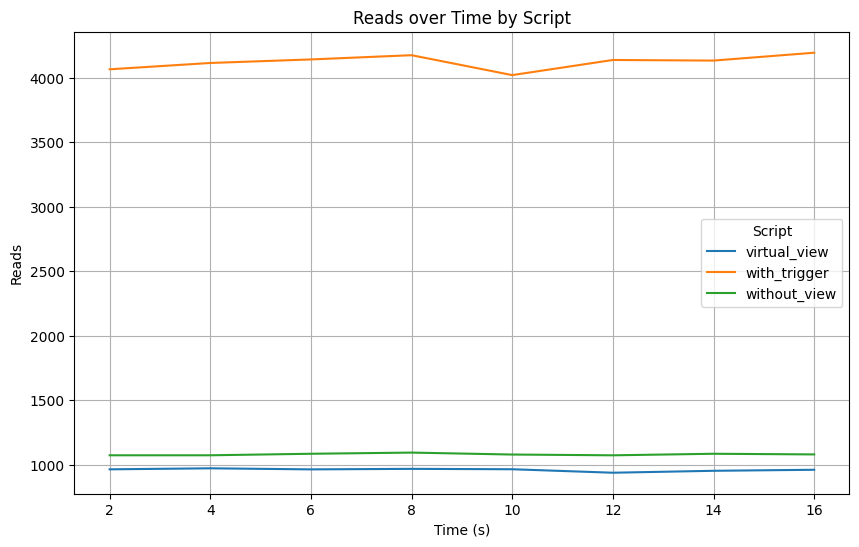
\includegraphics[width=\textwidth]{PNGs/Script/Views/view-comparison/Reads}
    \end{subfigure}
    \hfill
    \begin{subfigure}[t]{0.48\textwidth}
        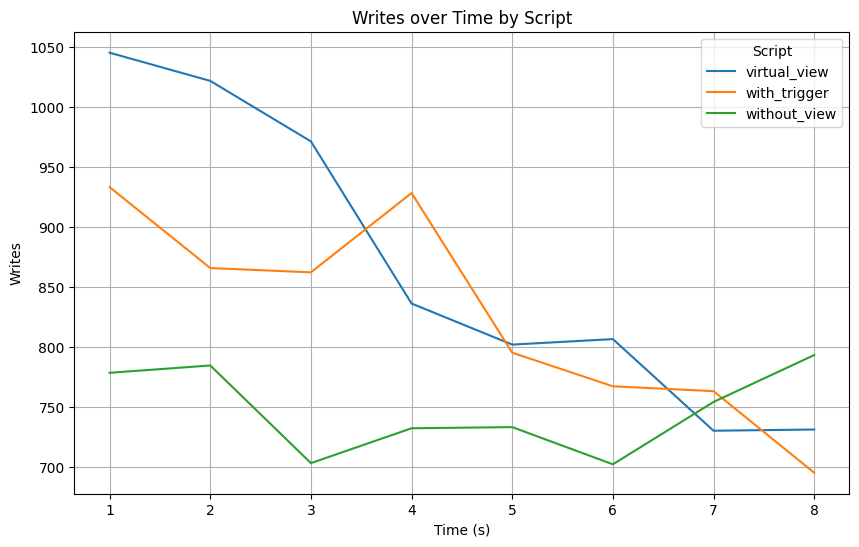
\includegraphics[width=\textwidth]{PNGs/Script/Views/view-comparison/Writes}
    \end{subfigure}
    \vspace{-20pt}
    \caption[Views: Keine View, virtuelle View und Ansatz mit Triggern]{Vergleich zwischen keiner View, der virtuellen View und dem Ansatz mit Triggern in MySQL}
    \label{fig:view-comparison-comp-metric}
\end{figure}
\vspace{-12pt}

Bei dem zweiten Vergleich sehen wir zuallererst einen sehr deutlichen Performanceunterschied beim Ansatz mit den Triggern zwischen Postgres und MySQL\@.
Begründet werden kann dieser Unterschied mit den verschiedenen Vorteilen des jeweiligen Datenbankmanagementsystems und dessen Umgebung.
Wir haben beide Systeme mit dem gleichen Ansatz gebenchmarkt, damit wir die Implementierung der nativen materialisierten Sicht, die nur in Postgres möglich ist, besser vergleichen zu können.
Denn die Ergebnisse der nativen Implementierung sind in Bezug auf die Abfragegeschwindigkeit tatsächlich am performantesten und die Anzahl an Aktualisierungen (\ref{lst:refresh-materialized-view}) hat dabei keinen Einfluss.
Anders hingegen sieht es bei der Einfüge-Geschwindigkeit aus, da dort die Implementierung, die nach jedem Insert-Befehl aktualisiert nicht am schnellsten, sondern am langsamsten ist.
Der Vergleich zwischen den DBMS fällt wieder schwer, da die Unterschiede zwischen \texttt{with\_trigger} und \texttt{with\_trigger\_postgres} sehr groß sind (etwa um Faktor 2--3).
Damit wird noch einmal deutlich wie stark die Einfügedauer bei den materialisierten Sichten von der Anzahl an Refreshs abhängig ist, da \texttt{mat\_view\_refresh\_every} unterhalb der Performance von \texttt{with\_trigger} liegt.
In unserem Beispiel ist die einmalige Aktualisierung der Sicht besser als das Verwenden der Trigger in Postgres.

\begin{figure}[H]
    \centering
    \begin{subfigure}[t]{0.48\textwidth}
        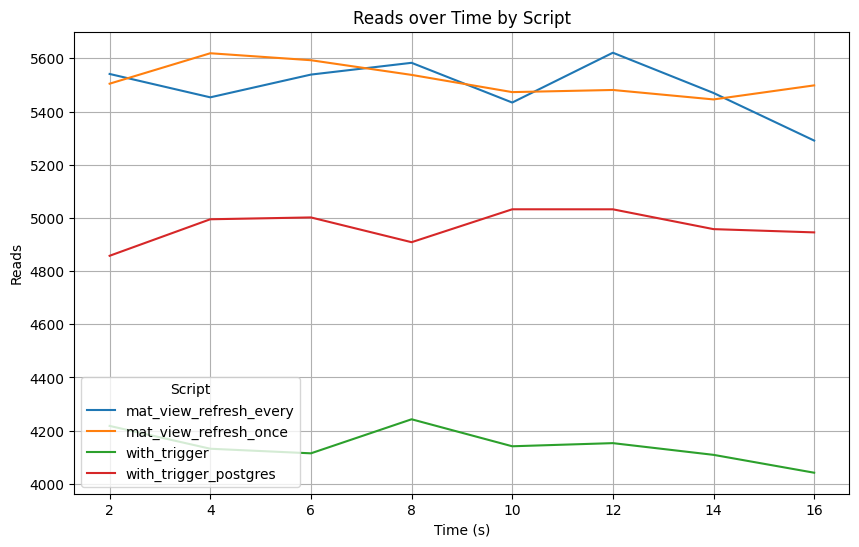
\includegraphics[width=\textwidth]{PNGs/Script/Views/mat-view-comparison//Reads}
    \end{subfigure}
    \hfill
    \begin{subfigure}[t]{0.48\textwidth}
        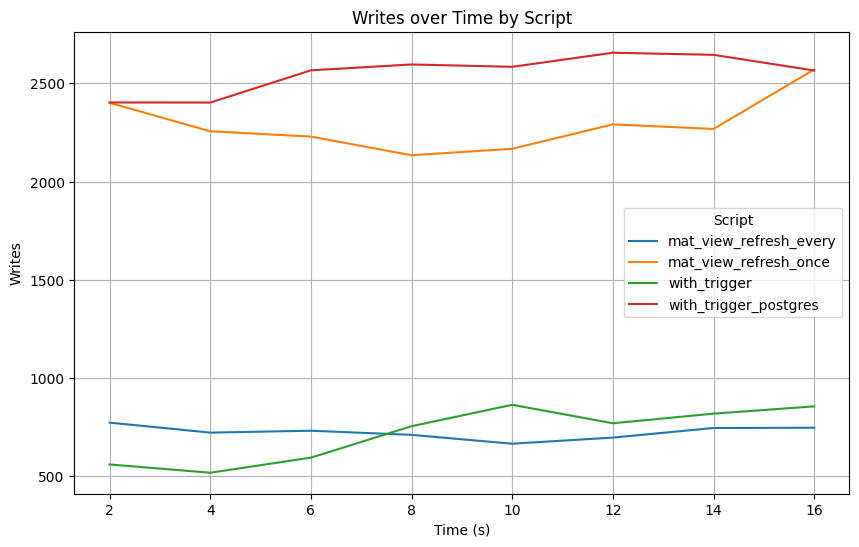
\includegraphics[width=\textwidth]{PNGs/Script/Views/mat-view-comparison/Writes}
    \end{subfigure}
    \vspace{-20pt}
    \caption[Views: Beide Triggeransätze sowie materialisierte Sicht]{Vergleich zwischen Triggeransatz in MySQL und Postgres, sowie zwei nativen Implementierungen in Postgres }
    \label{fig:mat-view-comparison-comp-metric}
\end{figure}
\vspace{-12pt}

Es lässt sich also zusammenfassen, dass virtuelle Sichten keine Auswirkungen auf die Performance haben.
Dies ist im eigentlichen Sinne aber auch nicht der Absicht der virtuellen Sicht, denn sie ist besser geeignet, um beispielsweise die Organisation der Rechte für unterschiedliche Nutzer der Datenbank zu gewährleisten.
Wenn man hingegen beispielweise in OLTP-Systemen die Notwendigkeit hat, dass man aggregierte Daten häufig zu der Analyse von bestimmten Daten benötigt, dann sind materialisierte Sichten nützlich.
Man sollte allerdings vor allem die Performanceauswirkungen von diesen Sichten nicht unterschätzen und sich gut überlegen, wie häufig und zu welcher Zeit die Daten aktualisiert werden müssen.